\section*{Introduction}\label{sec:intro}

%The investigation of an interplay between geometry and topology of the order parameter has become one of the key research fields in the modern soft and solid state physics, as it provides insight on the modification of material responses by geometrical tailoring. This result provides means both for fundamental study and technological applications: the presence of curvature in a generic electronic system leads to the appearance of scalar and vector geometric potentials, that introduce anisotropic and chiral responses to the system, respectively. This allows to fabricate novel logical and signal elements, that will meet growing technological demands for the high-density energy efficient electronics. For instance, novel fundamental responses were observed in thin layers of superconductors~\cite{Tempere09,Ying17}, superfluids~\cite{Kuratsuji12}, nematic liquid crystals~\cite{Lopez-Leon11}, cell membranes~\cite{McMahon05}, semiconductors~\cite{Gentile15,Ortix15}, and magnetism~\cite{Streubel16}. {\color{red} $\Leftarrow$ Do we need this paragraph? I think D. Sheka and D. Makarow will say something similar in the main introduction or preface.}

%Recent advances in the fabrication of curvilinear magnets \cite{Streubel16a,Fernandez17,Ball17,Sanz-Hernandez18,Huth18,Huth20,Sanz-Hernandez20} raises the question of the influence of curvature on statics and dynamics of a magnetization. For spintronic devices the geometrically induced potentials arising from curved shapes gain practical importance. For example, designs of these devices require wires with curvilinear segments, e.g. vertical U-shaped configuration increases the storage density of the potential magnetic racetrack memory devices~\cite{Parkin08,Zhang15}.

The purpose of this section is to introduce the general theory for the description of the flat curved one-dimensional~(1D) systems. The described methods are valid for systems with non-zero local curvature~(curved wires and narrow ribbons), and can not be used for description of boundary effects, e.g.  stabilization of vortex and antivortex in magnetically soft disk~\cite{Shinjo00} and astroid~\cite{Shigeto02} geometries, respectively.

%==================================================================\
\begin{figure}[t]
	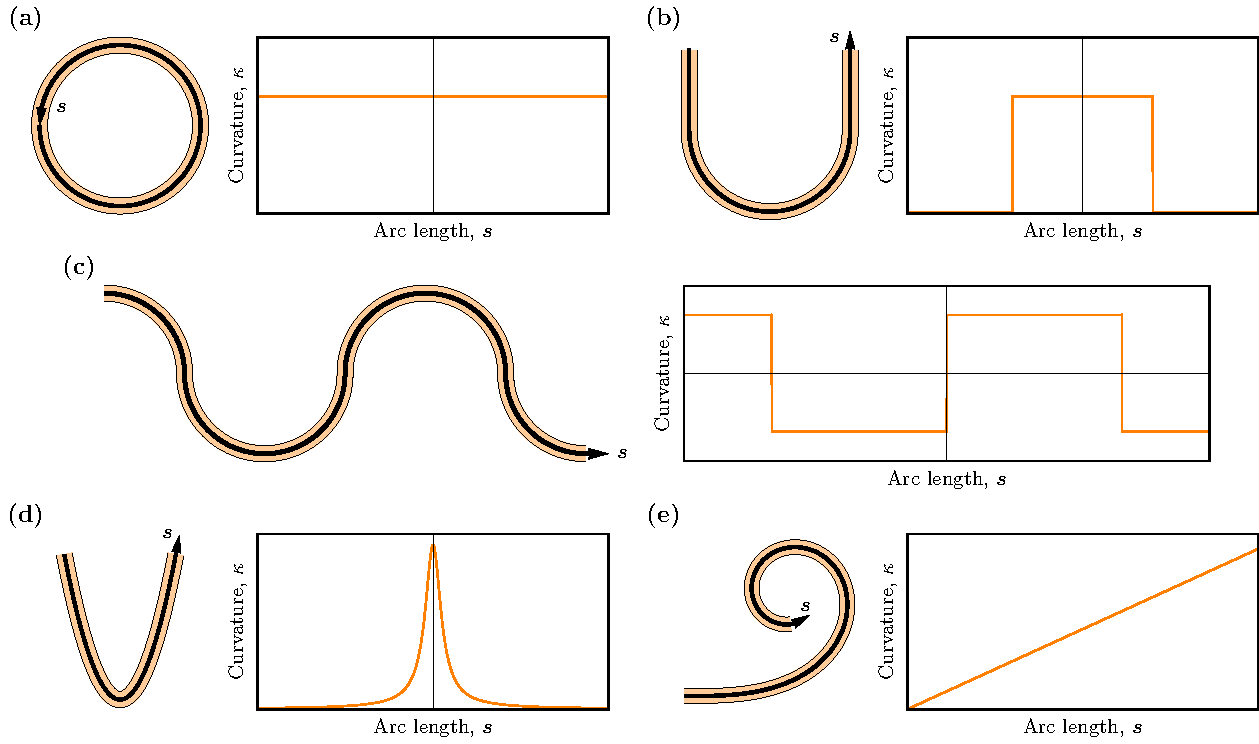
\includegraphics[width=\textwidth]{fig_geometries_n_curvatures}
	\caption{\label{fig:Geometries_n_curvatures}%
		\textbf{Schematics of flat curvilinear geometries and their curvature distributions.} (a) Circular ring with constant curvature. (b) Nanostripe with individual circular segment, which correspond to the box-function spatial profile of curvature. (c) Meander-like nanowire constructed from repeated semicircles of same radius $R$. The spatial distribution of the curvature of such a wire is the square-wave function. (d) Parabolic nanostripe with localized curvature distribution. (e) Euler spiral with constant non-zero gradient of the curvature along the stripe.}
\end{figure}
%==================================================================/

In the present Chapter, we will limit ourselves to the description of various flat curvilinear magnetic geometries, i.e. planar geometries within $xy$ plane and zero torsion [see Fig.~\ref{fig:Geometries_n_curvatures}], and corresponding curvature-induced effects. Namely, we will address the impact of curvature on magnetic subsystem for the following geometries:
\begin{itemize}
	\item \textbf{Nanorings} as geometries with constant curvature, see Fig.~\ref{fig:Geometries_n_curvatures}(a);
	\item \textbf{Nanowire with circular segment} and box-function curvature profile, see Fig.~\ref{fig:Geometries_n_curvatures}(b);
	\item \textbf{Meander-like shape nanowire} with the square-wave curvature distribution, see Fig.~\ref{fig:Geometries_n_curvatures}(c);
	\item \textbf{Parabolic nanowires} with localized curvature distribution, see Fig.~\ref{fig:Geometries_n_curvatures}(d);
	\item \textbf{Euler spirals} with constant gradient of the curvature along the stripe, see Fig.~\ref{fig:Geometries_n_curvatures}(e).
\end{itemize}
Magnetic effects associated with presence of curvature and torsion in three-dimensional curvilinear magnetic systems will be discussed elsewhere.